\section{Knowledge Based Backbone Dihedral Penalty}
\label{section:unsorted/rfs}
Though the systematic search method of sampling closed loops uses a rotamer of $(\phi,\psi)$ backbone dihedral pairs, it is still possible for amino acids to fall outside of the permitted dihedral space.
These unfavored dihedrals can be introduced at least two different ways:
\begin{enumerate}
\item If the loop closure criteria is approximate superposition of a single atom, any dihedrals containing this atom can fall outside the allowed area, and the angle centered at the atom can also be very high energy,
\item If the initial loop conformation, including the predicted side chains, is strained, it is possible for any loop dihedrals to be push out of the permitted space.
\end{enumerate}
Because some loop closure techniques, such as random tweak, and the systematic search implemented in PLOP, possibly introduce disfavored dihedrals, many loop sampling techniques apply filtering criteria to remove these dihedrals \cite{fine1986predicting,shenkin1987predicting}.

It has also been observed that sequential $(\phi, \psi)$ pairs are correlated in protein structure.
This correlation has been used in PLOP to create a dipeptide library which is smaller than the product of the sequential peptide libraries.
This has the effect of accelerating sampling by reducing sampling in areas of the $(\phi_{1}, \psi_{1}, \phi_{2}, \psi_{2})$ space which are unlikely to be occupied.
Using this information the predictive ability of PLOP was extended from thirteen to seventeen residue loops \cite{zhao2011progress}.

\begin{figure}[h]
    \centering
    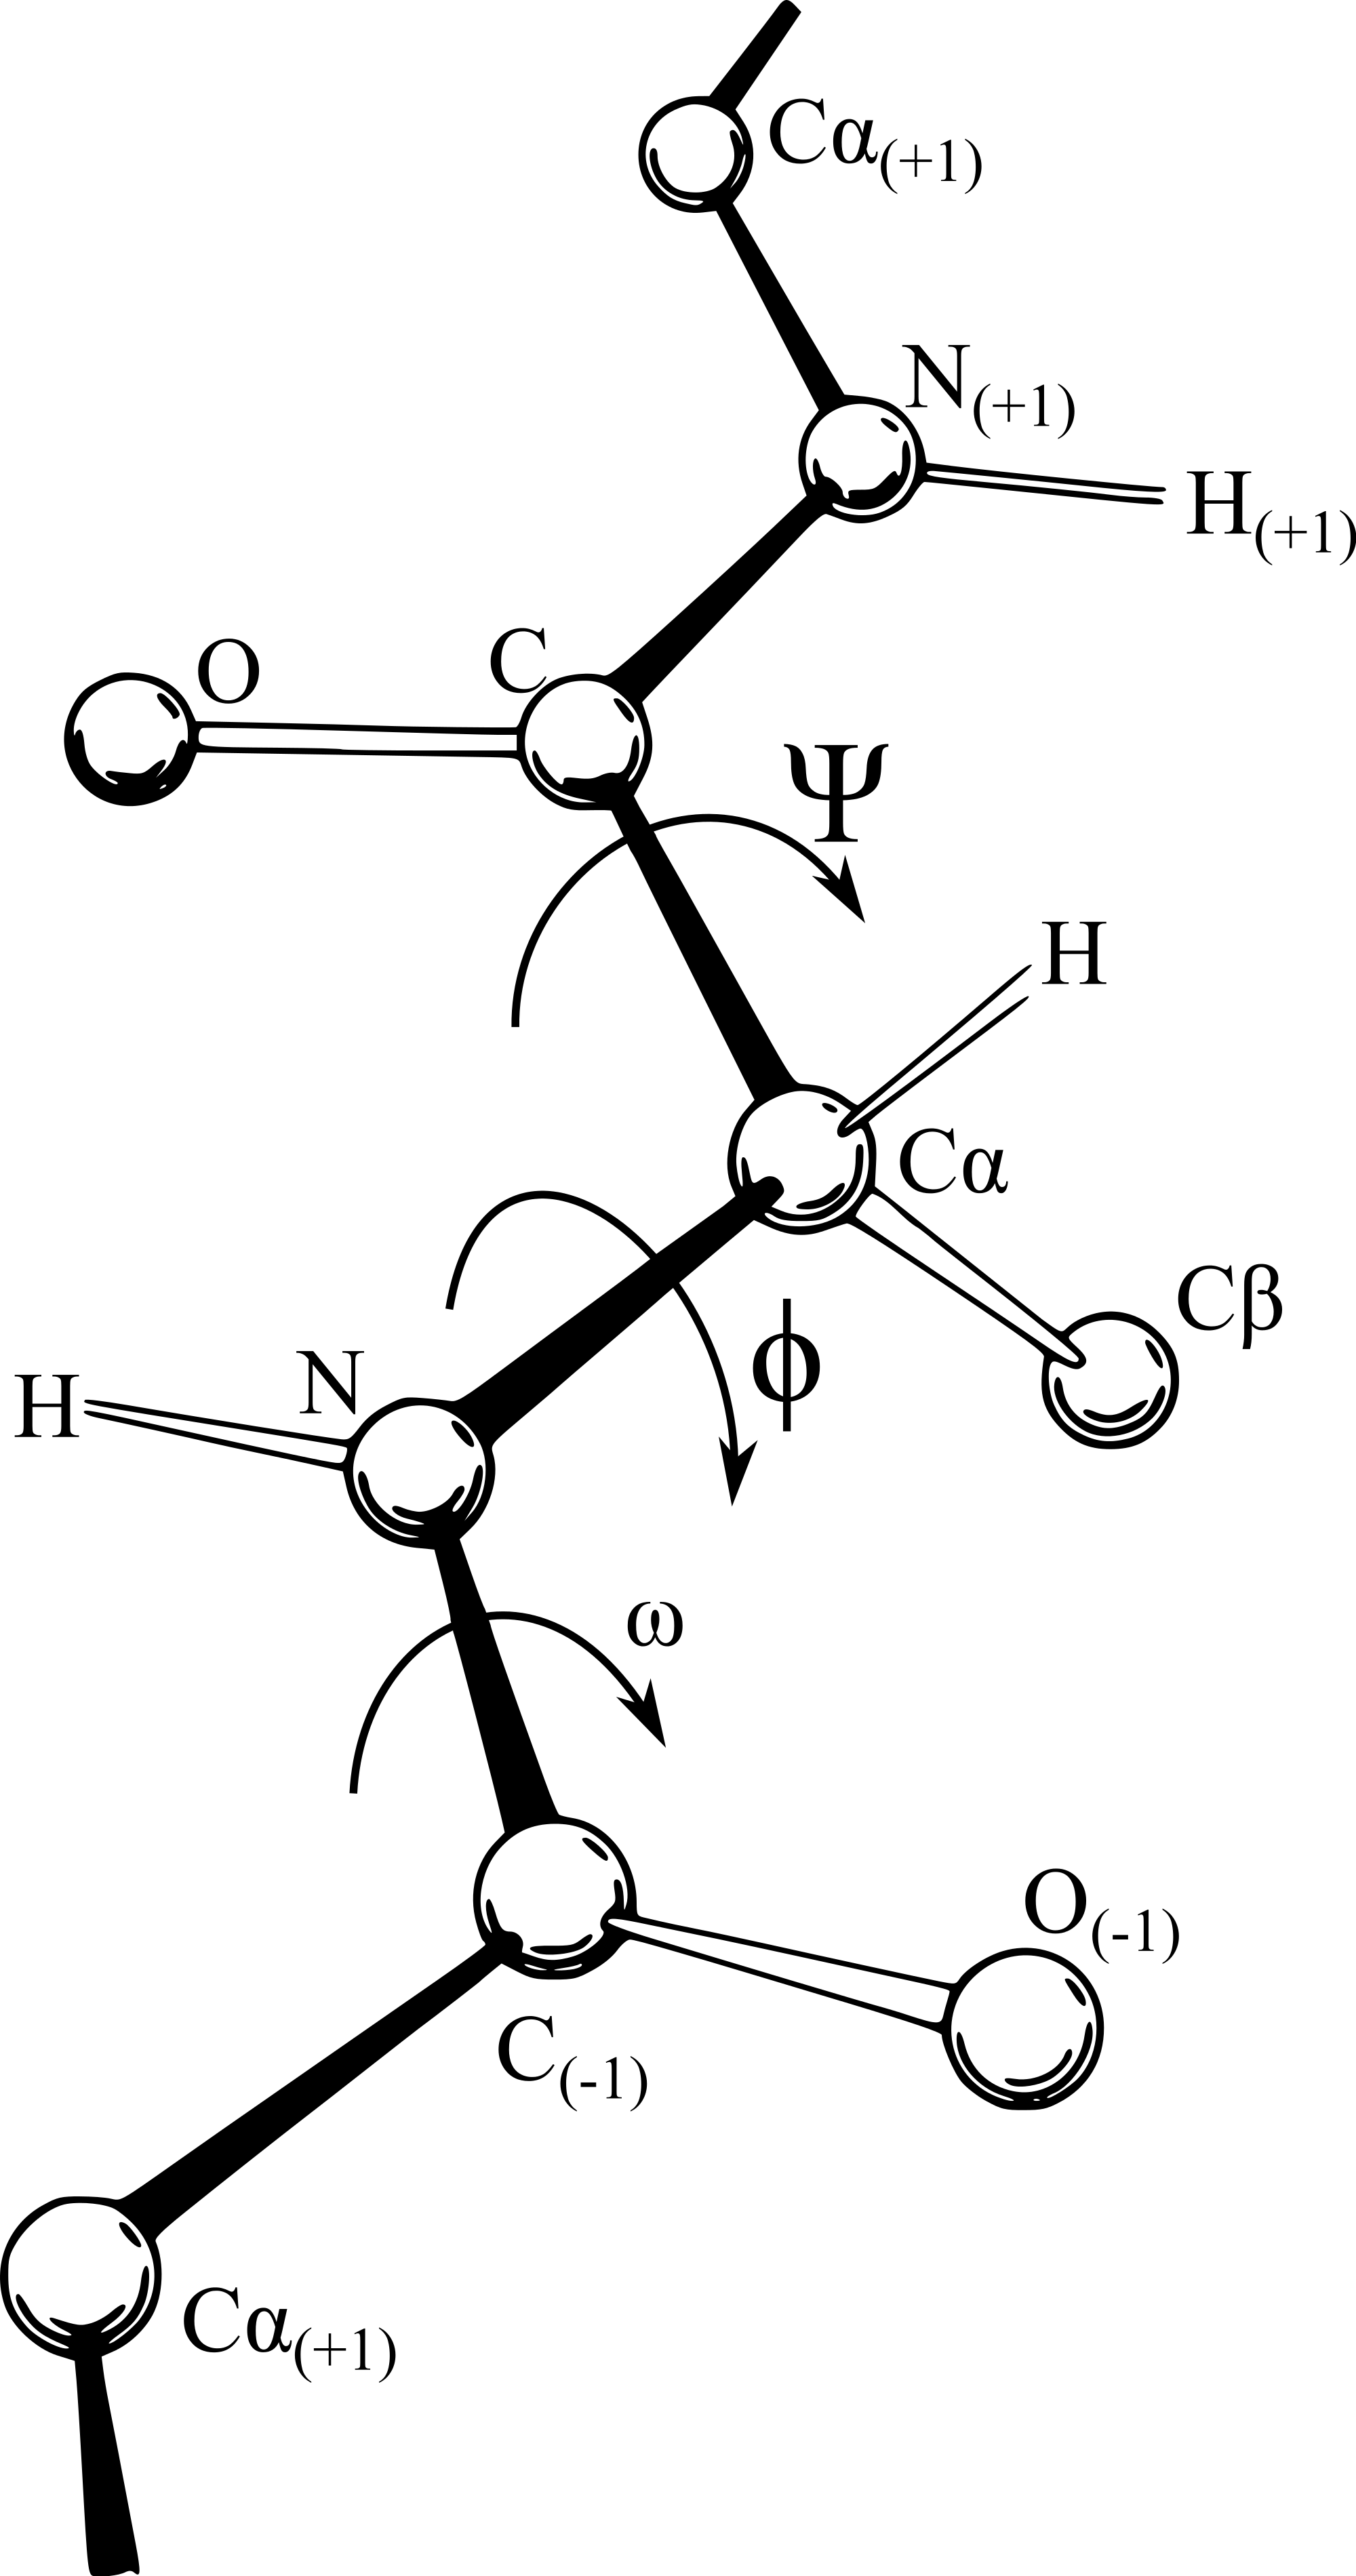
\includegraphics[width=0.65\textwidth,height=0.3\textheight,keepaspectratio]{figures/backbone_labels.png}
    \caption{Labels assigned to protein backbone dihedrals.
The diehedrals used in the knowledge based penalty term are $(\phi_{1}, \psi_{1}, \omega_{1}, \phi_{2}, \psi_{2})$}.
    \label{figure:backbone_labels}
\end{figure}

\begin{figure}[h]
    \centering
    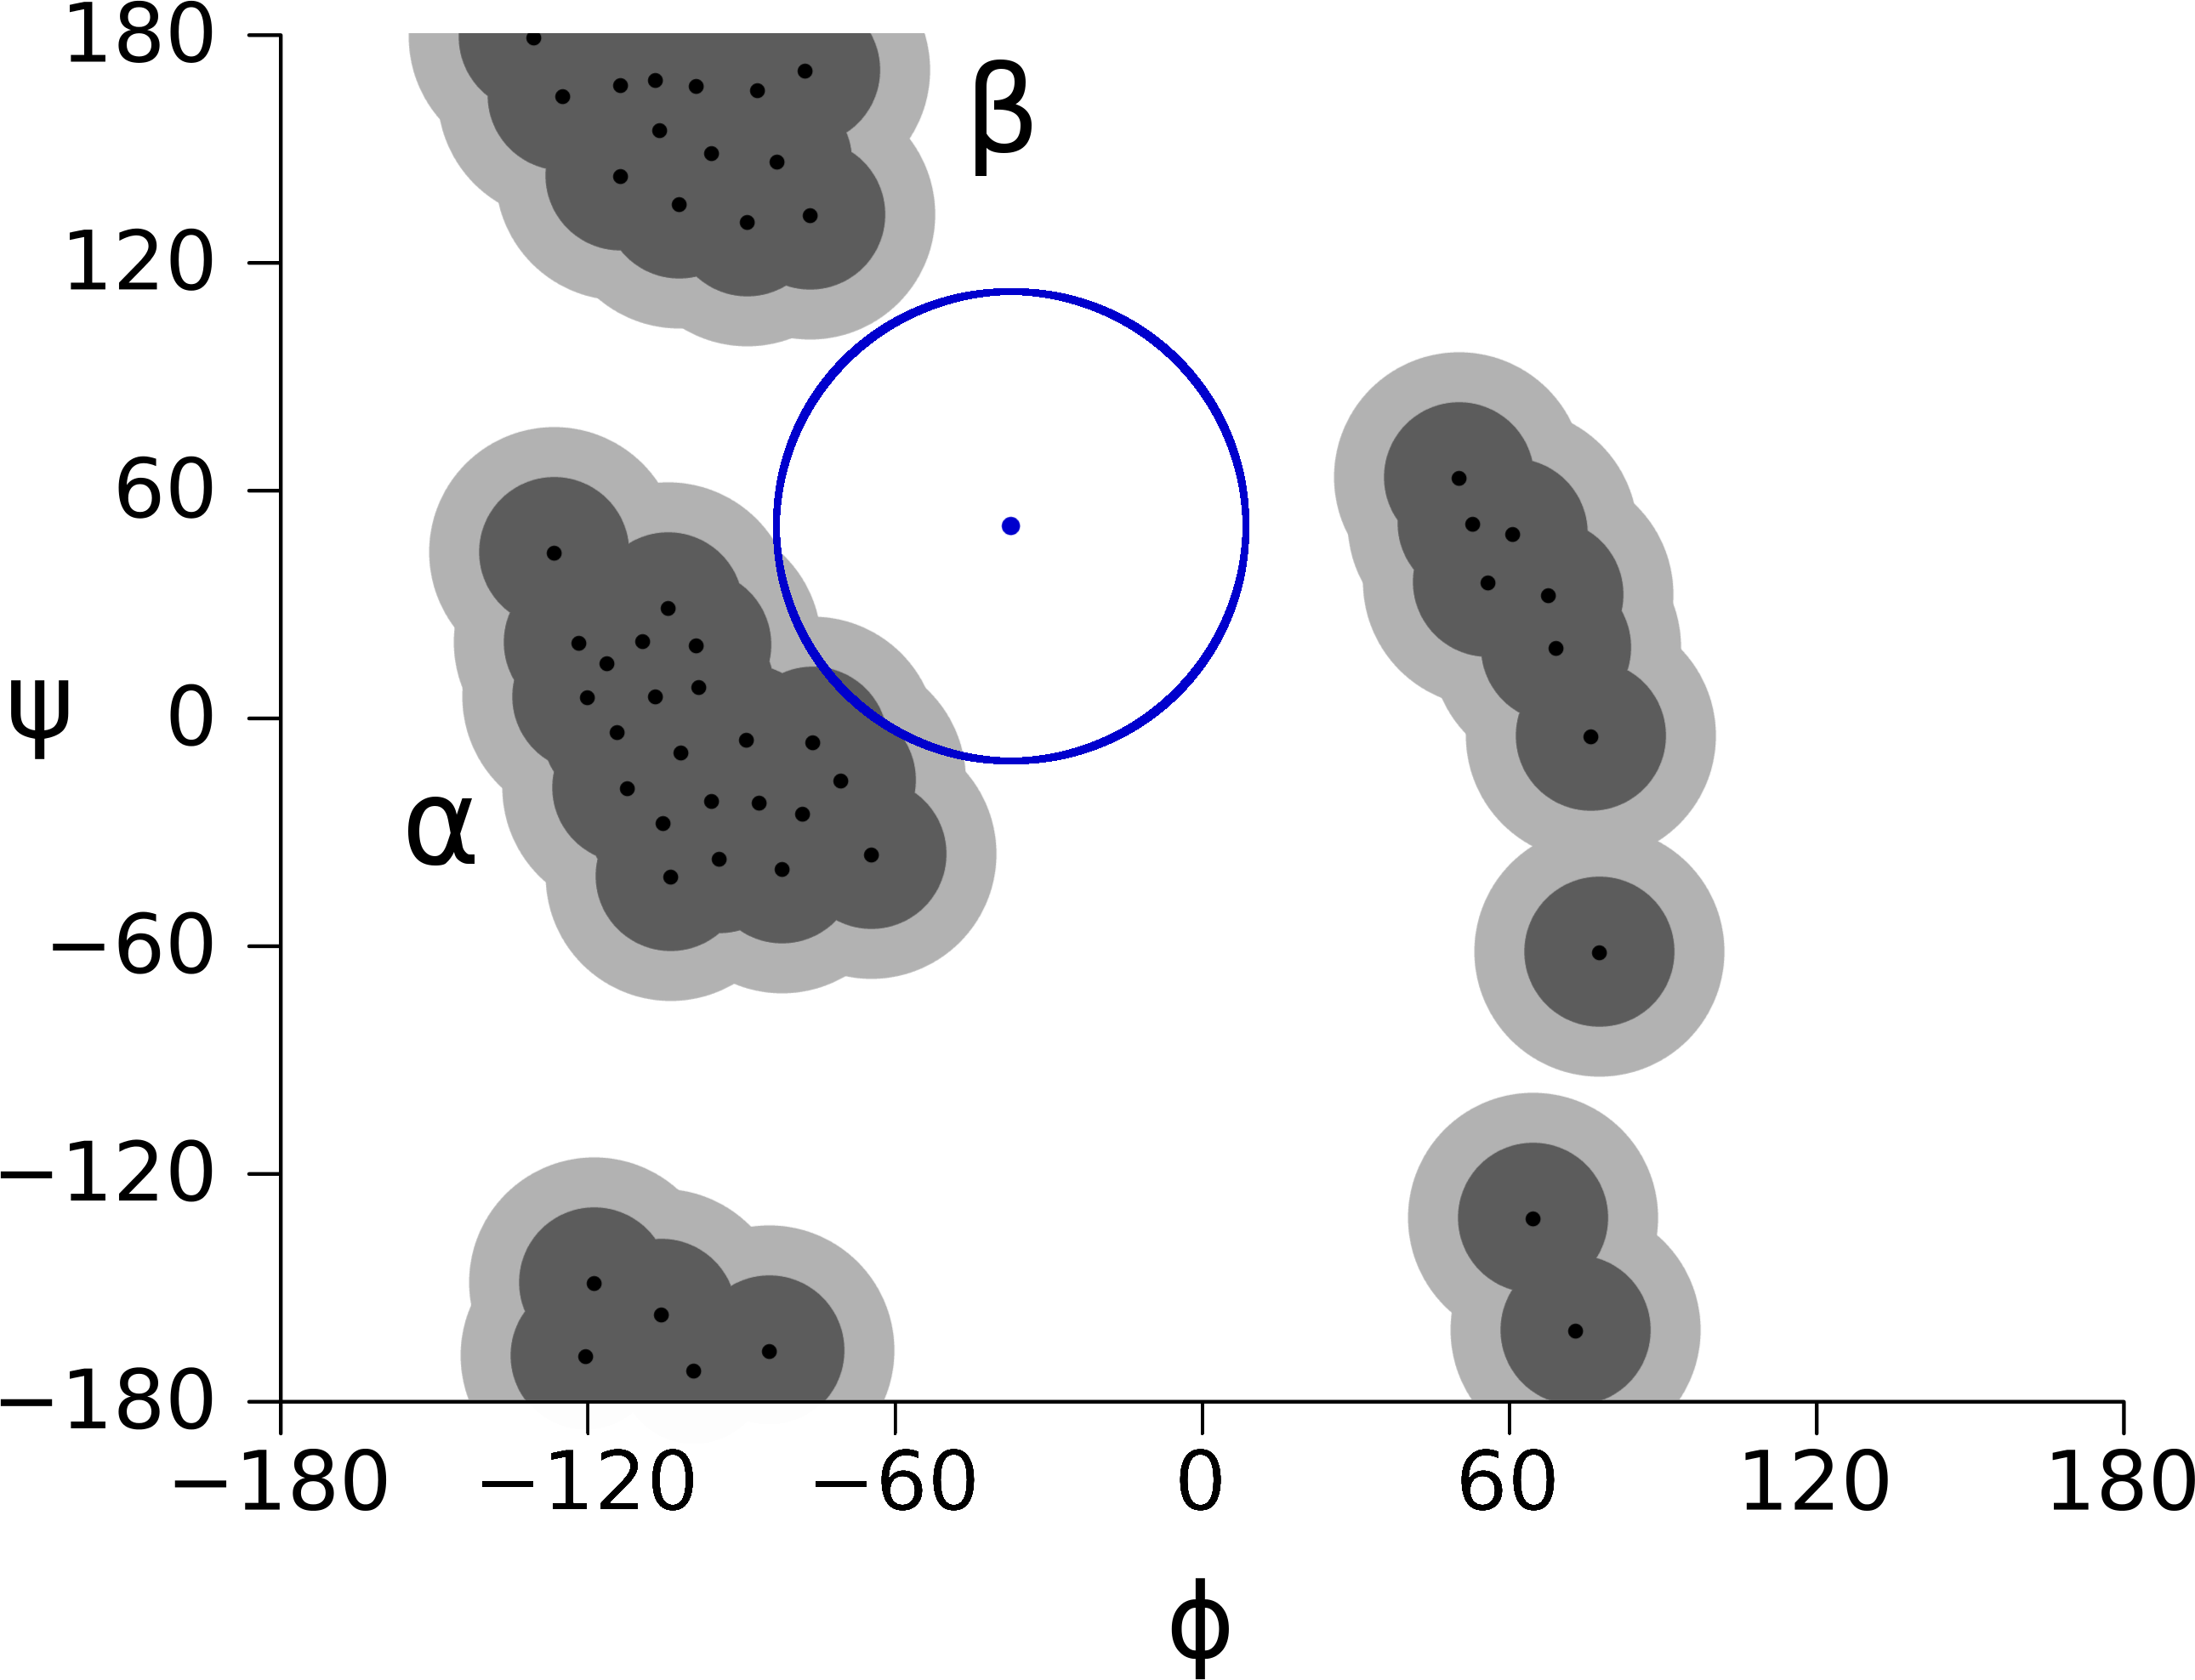
\includegraphics[width=0.8\textwidth,height=0.5\textheight,keepaspectratio]{figures/rfs_ex.png}
    \caption{A simulated Ramachandran plot illustrating a similar scoring surface in two dimensions.
Dark gray areas, or those very near a library rotamer are considered native like and are never penalized.
Light gray areas, are pseudo-native like and are penalized at a linear rate if fewer than 30 library rotamers are found within a Euclidean distance $D$ of the conformation.
Rotamers in the white area are penalized according to how many library rotamers are contained within the distance $D$ of the rotamer, illustrated by a blue circle in the figure.
If 30 or more library rotamers are found within the blue circle the conformation is not penalized at all.
If the blue circle contains between 5 and 30 library rotamers the conformation is assigned a penalty proportional to the distance from the nearest rotamer.
If the blue circle contains fewer than 5 library rotamers the penalty is proportional to the square of the distance to the nearest rotamer.}
    \label{figure:rfs_plot}
\end{figure}

Using a similar idea we sought to filter proposed loop conformations which contained unfavorable $(\phi_{1}, \psi_{1}, \omega{1}, \phi_{2}, \psi_{2})$ combinations.
The dipeptide rotamer frequency-based scoring term employed a dipeptide rotamer library constructed from {\textapprox}7500 high-quality PDB structures.
Frequently occurring rotamers, corresponding to very populated regions in the higher dimensional equivalent to the Ramachandran plot are weighted according to their frequency in this subset of the PDB.

Two criteria determine whether a penalty will be applied to the dipeptide: 
\begin{enumerate}
\item if the Euclidean distance between the loop dipeptide and the nearest rotamer in the library is greater than a certain, empirically determined cutoff
\item if the total population of rotamers within a set radius of the loop dipeptide is below a certain threshold The form of this penalty term, its implementation, and its successes in improving loop prediction in crystal structure and homology model environments will be discussed in detail in an upcoming publication.
\end{enumerate}

